\documentclass{article}
%\usepackage[cyr]{aeguill}
\usepackage[utf8]{inputenc}
\usepackage[T1]{fontenc}
\usepackage[francais]{babel}
\usepackage{amsmath}
\usepackage{fancyhdr}
\usepackage{amsfonts}
\usepackage{makeidx}         
\title{Projet GM4 : Programme de détection de spam}
\usepackage[pdftex]{graphicx}
\author{Jean Prost \and Edouard Gouteux \and Lucas Potin} 
 
\begin{document}
\maketitle
 
% une série de blocs comme celui qui suit
\section{Introduction à la méthode}

L'idée principale de la méthode est que l'on peut prédire de manière correct si un mail est un spam ou non, ceci uniquement à l'aide d'une combinaison bayésienne de probabilités de mots présents dans le mail traité. L'idée est de faire ressortir les mots ( ou extraits de code html ) qui nous donnent un indice significatif sur la probabilité qu'un mail soit un spam ou non, et ceci de manière la plus efficace possible. 

\section{Pré-traitement}

\subsection{La phase de pré-traitement d'un corpus ou d'un mail}

Nous allons appliquer notre algorithme sur un texte comprenant uniquement des mots ou expressions traitables, c'est à dire n'ayant pas une taille trop significative ( dans ce cas il y aurait peu de chance que l'expression serve lors du calcul des probabilités, puisque cette expression n'apparaitrait qu'une seule fois). Nous devons donc effectuer un pré-traitement du texte brut (code html compris ) avant le "vrai" traitement afin "d'épurer" le texte brut de tout ce qui nous est inutile pour le calcul des probabilités de chaque mot. 
Pour se faire, il nous faut extraire les indices les plus significatifs du code html ( par exemple les couleurs très criardes utilisées pour les publicités ) ou encore des termes qui sont redondantes dans les spams. Le reste sera supprimé afin de ne garder que le nécessaire pour le calcul du nombre d'occurrence de chaque jeton. 

\subsection{Détail de la phase de pré-traitement}

%%je vais approfondir 
On balaie l'intégralité du texte, y compris les en-têtes, les scripts HTML et JavaScript intégrés, de chaque message de chaque corpus. On considère  que les caractères alphanumériques, les tirets, les apostrophes et les signes en dollars font partie des jetons, et que tout le reste est un séparateur de jetons. On ignore les jetons qui sont tous des chiffres et également les commentaires html, sans même les considérer comme des séparateurs de jetons.

De chaque pré-traitement sur un corpus résulte une table de hachage contenant un ensemble de jetons avec pour chaque jeton le nombre d'apparition dans le corpus.

\section{Phase de traitement principal}

\subsection{Le calcul des probabilités}

%%je vais approfondir
Après avoir trié et répertorié nos jetons, nous obtenons un ensemble de jeton avec leur nombre d'occurrence dans chacun des corpus. Nous pouvons extraire de ces données une probabilité pour chaque jeton ( comprise entre 0 et 1 )  

Le code est le suivant : \\

(let ((g (* 2 (or (gethash word good) 0)))\\
      (b (or (gethash word bad) 0)))\\
   (unless (< (+ g b) 5)\\
     (max .01\\
          (min .99 (float (/ (min 1 (/ b nbad))\\
                             (+ (min 1 (/ g ngood))   \\
                                (min 1 (/ b nbad)))))))))\\

\subsection{Données d'entrainements}

Avant de pouvoir appliquer notre algorithme à un mail afin de savoir si c'est un spam ou non et de pouvoir faire des tests avec des échantillons de mails spams et/ou non-spam, 
nous avons besoin de données d'entrainement. Ces données d'entrainement sont nécessaires afin que notre algorithme "apprenne" en quelque sorte à détecter les spams. ( voir partie sur le pré-traitement et sur le calcul des probabilités ) 
Pour obtenir un bon taux de prédiction, nous avons besoin d'un corpus de mail d'apprentissage conséquent. En effet, 4000 mails spam et 4000 non spam serait l'idéal.

\section{La prédiction}

Après avoir effectué les étapes précédentes, nous pouvons commencer à prédire si un mail sera un spam ou non à l'aide de notre algorithme. Pour cela, un pré-traitement est déjà appliqué au mail afin de ne laisser que ce qui sera compréhensible par l'algorithme. L'algorithme parcours le mail et répertorie les jetons présents à l'intérieur de celui-ci. Enfin, nous usons des 15 jetons ayant les probabilités les plus significatives afin de déterminer si oui ou non notre mail est un spam. 

\section{Regard critique sur la méthode, problèmes}

Selon le créateur de cette méthode, il faudrait instaurer un 
"seuil" de filtrage afin de diminuer le nombre de faux spams (mails qui ne sont pas des spams mais qui sont répertoriés comme tel par l'algorithme). Car en effet, une personne préfère en général recevoir quelque spams dans sa boite mail que de voir un message important finir dans les courriers indésirables. 
%%je vais préciser la démarche
Avoir un bon algorithme de prédiction des spams peut être dangereux. En effet, si l'algorithme est très performant et que nous lui faisons trop confiance, nous pouvons passer à côté d'un mail important, ce qui présente un problème.

\section{Modélisation UML}

Les classes java utilisées pour l'implémentation de la méthode : \\
- Scanner : classe relative au traitement du texte, contient les méthodes permettant de remplir les différents types de table de hachage. \\
- Predicteur : classe qui permet de prédire si un mail est un spam ou non. \\
- Mail : classe contenant le mail sous forme d'un fichier texte.\\
- Corpus : Ensemble de mail. \\

2 types de Table de Hachage  :\\
- table contenant les mails (Non Spam / Spam).\\
- table contenant les probabilités basée sur l'apparition des jetons dans les mails spam/non spam.\\

\subsection{Diagramme des cas d'utilisation}

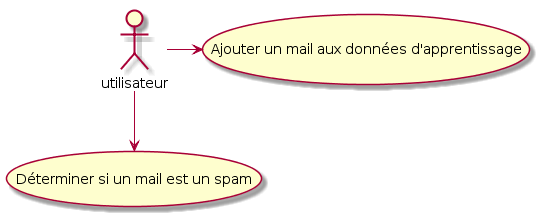
\includegraphics[scale=0.6]{diag_usecase.png}

\subsection{Diagramme de séquence}
On considère la situation ou, l'utilisateur souhaite connaître la probabilité estimée que son mail soit un spam.

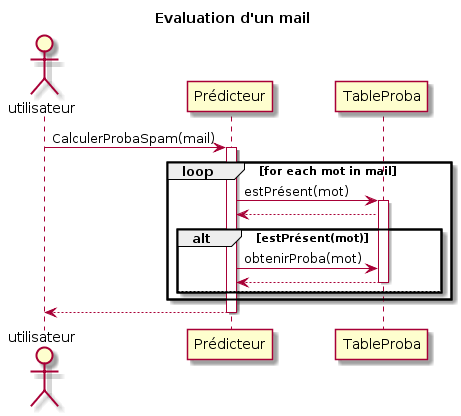
\includegraphics[scale=0.7]{diag_sequence.png}

\subsection{Diagramme de classe}

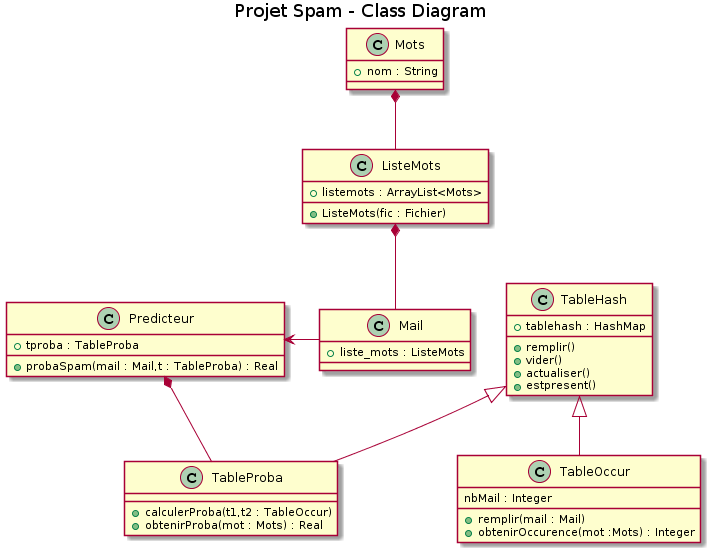
\includegraphics[scale=0.5]{diag_classe.png}

\end{document}